For training large neural networks you often need expensive hardware if you want to do it on your own. 
The way to do it these days is to use cloud services such as Google or Amazon to run the machine learning once you have prepared the dataset and the model. 
These services are often paid by the hour, but it's not expensive as long as you remember to shut it down after use, and only run it when you really need to.

Our dataset, however, only contains 55 participants and only a few days of activity measurements for each participant, 
so using a service to train the model would not be necessary. We decided to train them on one of our own personal computers, 
with an Nvidia GTX 1070. Our guess is that this GPU will do the job just fine. 
 
\section{Regression}

\begin{figure}
      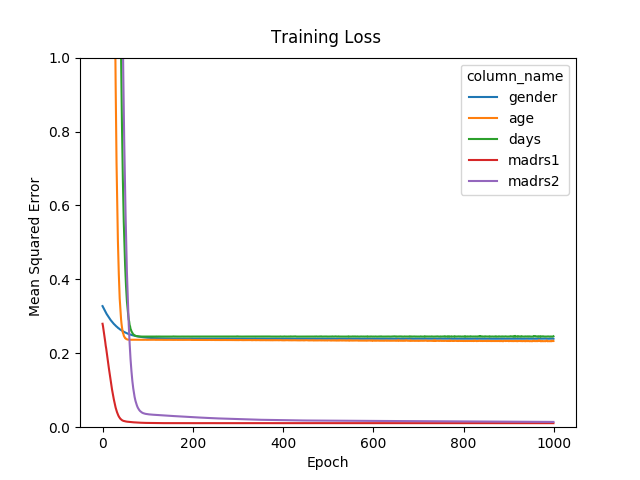
\includegraphics[height=9cm]{img/regression/results_kerasregressor_1k_epochs.png}
      \caption{Regression Training Loss (MSE) by Epoch}
      \label{figure:regression_training_loss}
\end{figure}

\begin{figure}
      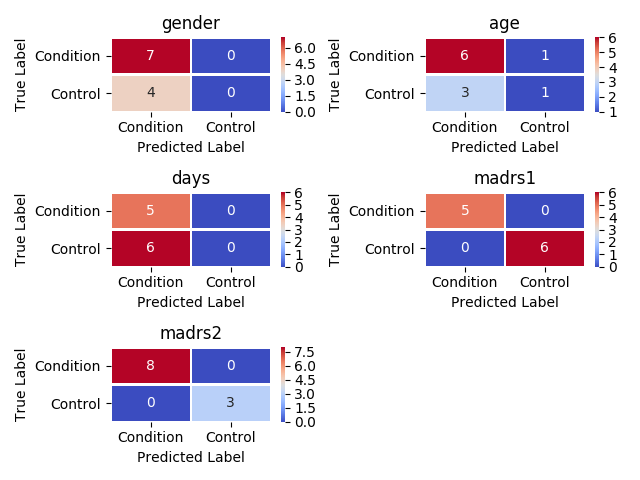
\includegraphics[height=8cm]{img/regression/confusion_kerasregressor_grouped.png}
      \caption{Confusion Matrices for Regression}
      \label{figure:regression_test_confusion}
\end{figure}

We ended up training the regression model \ref{code:regression_model} for 1000 epochs using a batch size of 16. Because of the simplicity of the model, 
1000 epochs did not take that much time and the training loss graph \ref{figure:regression_training_loss} shows that more epochs won't yield any better results. 
The loss does not reduce any more after the first 100 epochs for any of the columns. As we said earlier, we wanted the model to predict 
flawlessly based on the MADRS scores, and the loss results from training these are clearly better than for the other columns. 

We used the \textbf{train\_test\_split} function to create training and testing data, and because of how few rows there are in this dataset, 
we used an 80/20 split for training and testing data. 20\% of the dataset in the test data seemed to be good enough for this experiment 
because we wanted as many rows as possible to train on. Note that the data elements that were in the test and train splits were different for each column. 

\subsection{Results}

The confusion matrices \ref{figure:regression_test_confusion} displays the results when running the prediction on the test data (and then using it as classification). 
We said we wanted 100\% on all metrics for the MADRS score columns, and this is clearly achieved because the model guessed everything right. 
The other columns have these performance scores (using \textbf{condition} as positive and \textbf{control} as negative):

\begin{multicols}{2}
\subsection{Accuracy}
$ A = \frac{TP+TN}{TP+TN+FN+FP} $
\\\\
- \textbf{Gender}: $\frac{7+0}{7+0+4+0} = 7/11 \approx 63\%$\\\\
- \textbf{Age}: $\frac{6+1}{6+1+3+1} = 7/11 \approx 63\%$\\\\
- \textbf{Days}: $\frac{5+0}{5+0+6+0} = 5/11 \approx 45\%$\\

\subsection{Precision}
$ P = \frac{TP}{TP+FP} $
\\\\
- \textbf{Gender}:$ \frac{7}{7+0} = 7/7 = 100\%$\\\\
- \textbf{Age}: $\frac{6}{6+1} = 6/7 \approx 86\%$\\\\
- \textbf{Days}: $\frac{5}{5+0} = 5/5 = 100\%$\\

\subsection{Recall}
$ R = \frac{TP}{TP+FN} $
\\\\
- \textbf{Gender}: $\frac{7}{7+4} = 7/11 \approx 63\%$\\\\
- \textbf{Age}: $\frac{6}{6+3} = 6/9 \approx 67\%$\\\\
- \textbf{Days}: $\frac{5}{5+6} = 5/11 \approx 45\%$

\subsection{Specificity}
$ S = \frac{TN}{TN+FP} $
\\\\
- \textbf{Gender}: $\frac{0}{0+0} = 0/0$\\\\
- \textbf{Age}: $\frac{1}{1+1} = 1/2 = 50\%$\\\\
- \textbf{Days}: $\frac{0}{0+0} = 0/0$\\

\end{multicols}

\subsection{F1 Score}
$ F1 = 2 \cdot \frac{P \cdot R}{P + R} $
\\\\
- \textbf{Gender}: $2 \cdot \frac{1 \cdot 0,63}{1 + 0,63} \approx 77\%$\\\\
- \textbf{Age}: $2 \cdot \frac{0,86 \cdot 0,67}{0,86 + 0,67} \approx 75\%$\\\\
- \textbf{Days}: $2 \cdot \frac{1 \cdot 0,45}{1 + 0,45} \approx 62\%$\\

Looking away from the results of \textbf{madrs1} and \textbf{madrs2}, because they were obviously going to be good, these performance scores tell us that the model 
is good at predicting that someone is in the condition group (see precision). Other than that, we can't really learn that much from them. 
Also, we have undefined specificity for both gender and days because we don't have any predictions for the values required to calculate them. 

However, we learned a lot about machine learning and regression doing this experiment, and we look at it more like a warmup for the more complex models that we built 
for the next goals.

\section{1D CNN: Control vs Condition groups}

\subsection{Training and finding the optimal segment length}

Next up was our goal to classify whether a participant belongs to the control group or the condition group. 
As we said in the section about optimizing the model, the segment length is what we thought was going to impact the result the most.  
To test this theory, we trained the model to fit input data created with segment lengths of 1, 2, 4, 8, 16, 24, 48 and 96 hours. 

The input data was split using \textbf{train\_test\_split} so that the training data was 80\% of the total and the rest was going to be used for 
testing after the training was complete. Of the training data, 40\% was set to be used as validation data, which made it easy for us to tell if the model was 
learning from epoch to epoch or not. 

We did the training for each of the eight different input sets for ten epochs. To keep it simple, we used a batch size of 16 and the Adam optimizer 
with a default learning rate of 0,001 throughout this experiment. The primary objective here was to find the best segment length to use, and not to 
train the models to be perfect,  so these hyper-parameters seemed fine for this purpose. Our guess before we started with the experiment was that 
the more hours of data we used, the better, meaning that 96 hours of data in each segment was going to give us the best model (from what was possible with only ten epochs).

Looking at the history graphs \ref{figure:control_condition_10e} for how the training went epoch by epoch for each of the experiment's datasets, 
we noticed that the results were better when increasing the number of hours up to 48, and then it did not seem to be any better for 96 hours. 
This was the case for both training and testing, as the evaluation graphs (results after testing the model with the test-split) to the right also show straight lines from 
48 hours to 96 hours. The question was whether 48 hours was our magic number, or if we just needed to train it more.

To find the best segment length, we needed to experiment with more epochs. We reran the same experiment for 50 epochs, with 48, 72 and 96 hour long segments. 
However, from the results for that \ref{figure:control_condition_50e}, it's clear that nothing more was achieved with segments longer than 48 hours. 

The classifications for the models trained to fit 48-hour segments you can see in the confusion matrices \ref{figure:control_condition_confusion_matrix_48h} 
are close to perfect. The additional 40 epochs of training reduced the false positive classifications by a little bit, which was worth the time in our opinion as 
you want the value of wrong classifications to be as close to 0 as possible. For this relatively small dataset, we are happy with a 
classification model with scores above 99\% on all performance metrics previously discussed. 

\begin{figure}
      \begin{multicols}{2}
            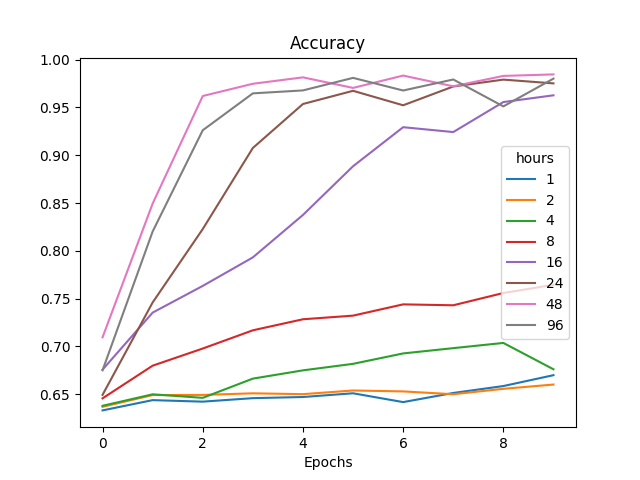
\includegraphics[height=5cm]{img/control_condition/plot_acc_train.png}
            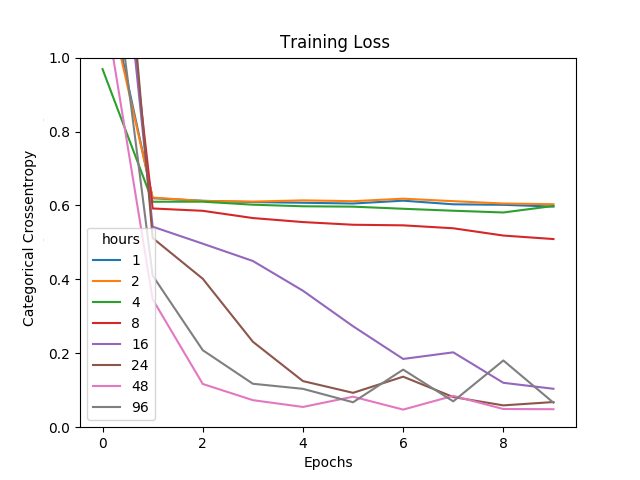
\includegraphics[height=5cm]{img/control_condition/plot_loss_train.png}

            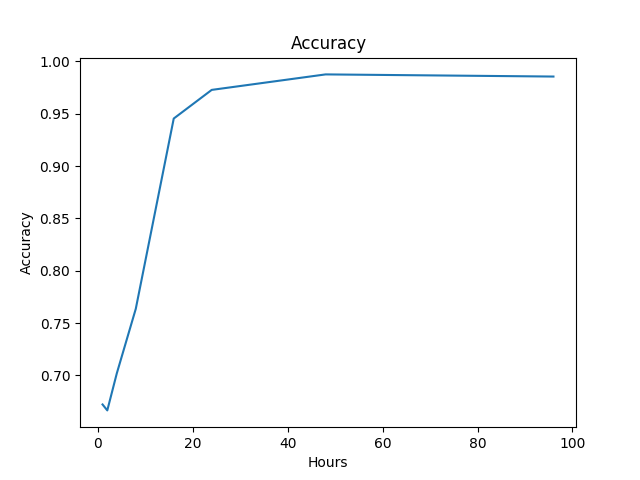
\includegraphics[height=5cm]{img/control_condition/plot_acc_eval.png}
            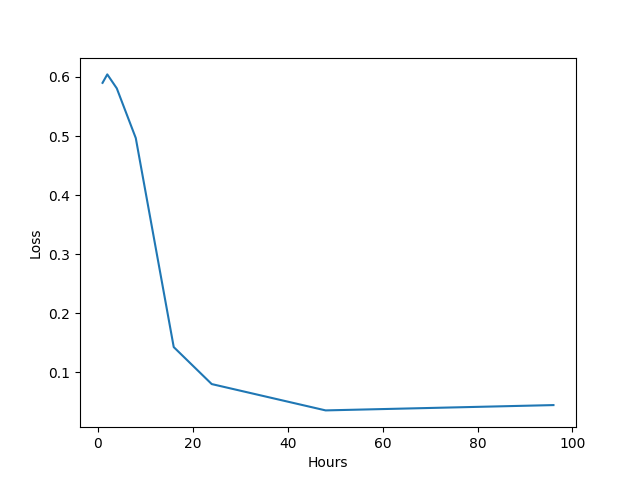
\includegraphics[height=5cm]{img/control_condition/plot_loss_eval.png}
      \end{multicols}
      \caption{Training (left) and testing (right) results (10 epochs)}
      \label{figure:control_condition_10e}
\end{figure}

\begin{figure}
      \begin{multicols}{2}
            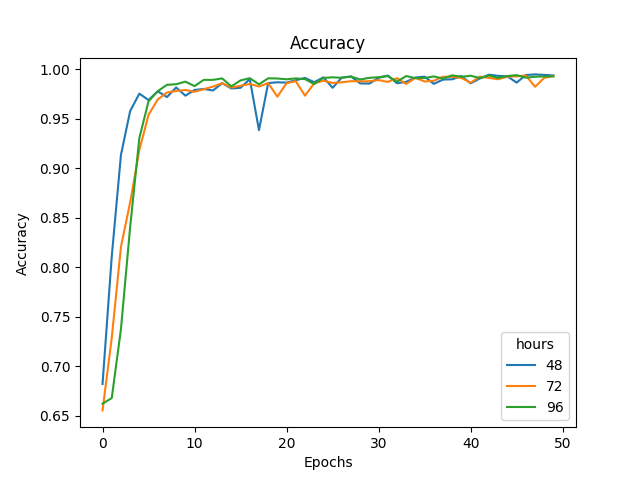
\includegraphics[height=5cm]{img/control_condition/plot_acc_train_50e.png}
            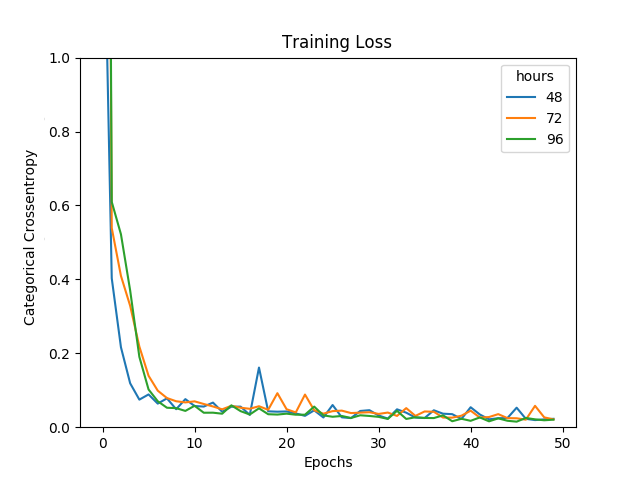
\includegraphics[height=5cm]{img/control_condition/plot_loss_train_50e.png}

            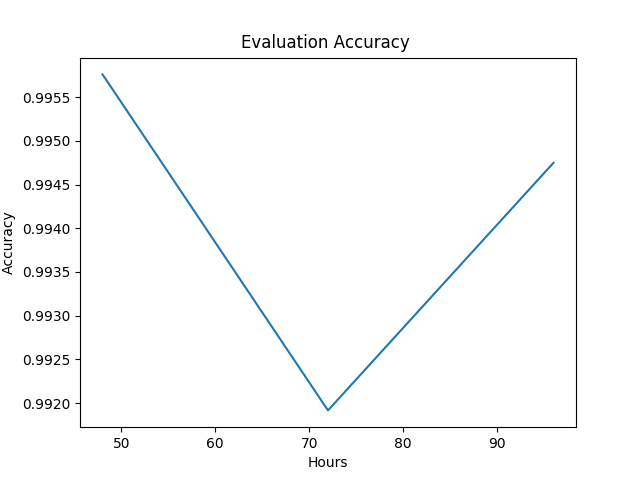
\includegraphics[height=5cm]{img/control_condition/plot_acc_eval_50e.png}
            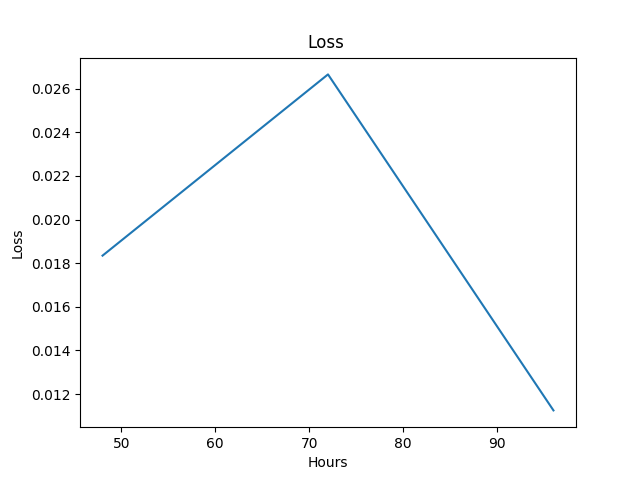
\includegraphics[height=5cm]{img/control_condition/plot_loss_eval_50e.png}
      \end{multicols}
      \caption{Training (left) and testing (right) results (50 epochs)}
      \label{figure:control_condition_50e}
\end{figure}

\begin{figure}
      \begin{multicols}{2}
            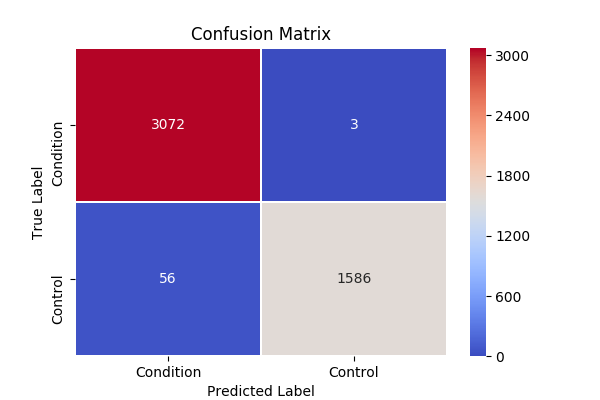
\includegraphics[height=4.5cm]{img/control_condition/conf_2880_60_10_32.png}
            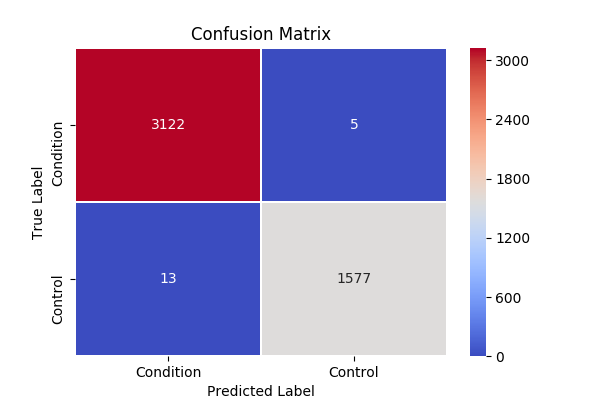
\includegraphics[height=4.5cm]{img/control_condition/conf_2880_60_50_32.png}
      \end{multicols}
      \caption{10 epochs (left) and 50 epochs (right) for 48 hour segments}
      \label{figure:control_condition_confusion_matrix_48h}
\end{figure}

%TP   FN   
%FP   TN

% \newpage IF NEEDED

\subsection{Performance metrics}

\subsubsection{Accuracy}
$ A = \frac{TP+TN}{TP+TN+FN+FP} = \frac{3122+1577}{3122+1577+5+13} \approx 99,6\%$

\subsubsection{Precision}
$ P = \frac{TP}{TP+FP} = \frac{3122}{3122+13} \approx 99,6\%$

\subsubsection{Recall}
$ R = \frac{TP}{TP+FN} = \frac{3122}{3122+5} \approx 99,8\%$

\subsubsection{Specificity}
$ S = \frac{TN}{TN+FP} = \frac{1577}{1577+13} \approx 99,2\%$

\subsubsection{F1 Score}
$ F1 = 2 \cdot \frac{P \cdot R}{P + R} = 2 \cdot \frac{0,996 \cdot 0,998}{0,996 + 0,998} \approx 99,7\% $

\subsection{Cross-validation}

To ensure that our model isn't overfitting and didn't get lucky when classifying the samples from the testing set, we proceeded to use 3-fold cross-validation. 
First, we split the dataset in two like before, into a train and test set (80/20 split here as well). Then we generated three folds containing training and 
validation parts, where for each fold a model was trained to fit the inputs. Each epoch the model was validated against the validation split. 
After training a model for a fold, we evaluated them by looking at the mean accuracy/loss against the global test split. If the accuracy was still high 
and the loss was still low, the model would have a good chance of doing correct classifications on unseen data.

To make this process quick, we trained the model for each fold only for ten epochs. The goal was to prove consistency in the model and not achieve high performance, 
so it seemed enough. As you can see in the cross-validation results \ref{figure:control_condition_5f_cv}, we have a mean loss of $0.06$ and a mean accuracy of $0.98$, 
which means that the model is consistently correct in most classifications.

\begin{figure}
    \begin{center}
        \begin{tabular}{|l|l|l|}
            \hline
            \bfseries Fold & \bfseries Loss & \bfseries Accuracy
            \csvreader[head to column names]{code/logs/control_vs_condition/5f_cv.csv}{}
            {\\\hline\fold & \loss & \accuracy}
            \\\hline
            \bfseries Mean & \bfseries 0.0629539173937511 & \bfseries 0.9809907427163319
            \\\hline
        \end{tabular}
        \caption{3-Fold Cross validation}
        \label{figure:control_condition_5f_cv}
    \end{center}
\end{figure}

\section{1D CNN: Depression Classes}

\begin{figure}
      \begin{multicols}{2}
            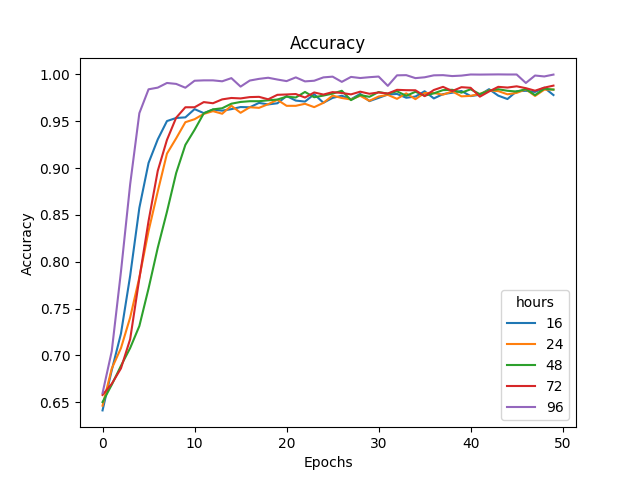
\includegraphics[height=5cm]{img/depression_class/plot_acc_train.png}
            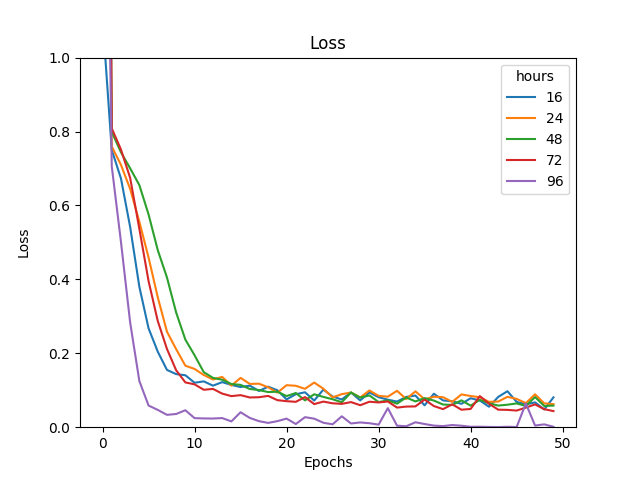
\includegraphics[height=5cm]{img/depression_class/plot_loss_train.png}

            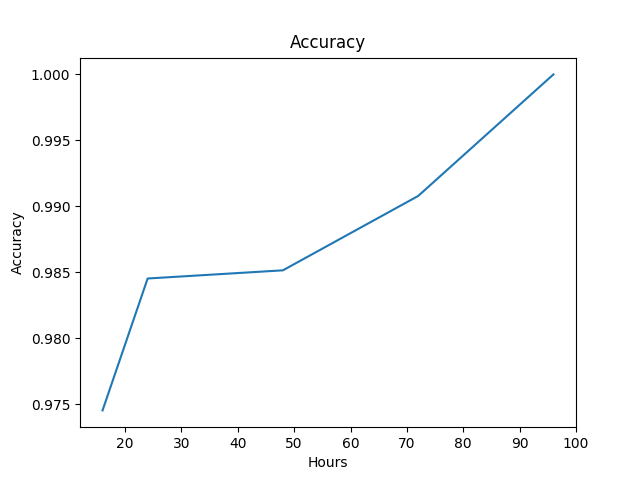
\includegraphics[height=5cm]{img/depression_class/plot_acc_eval.png}
            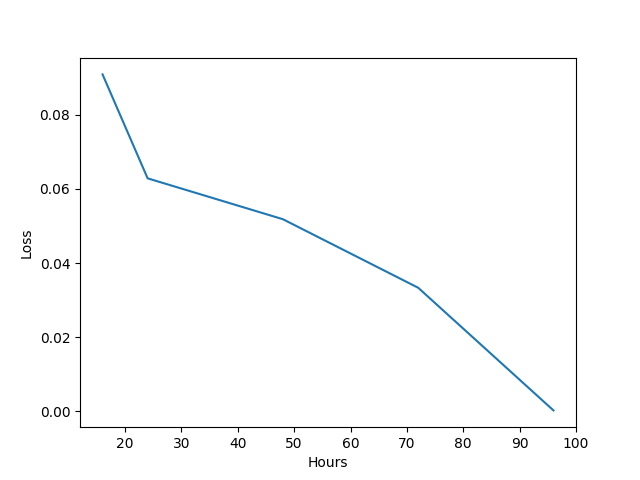
\includegraphics[height=5cm]{img/depression_class/plot_loss_eval.png}
      \end{multicols}
      \caption{Depression classes: Training (left) and testing (right) results (50 epochs)}
      \label{figure:depression_class_50e}
\end{figure}

\begin{figure}
      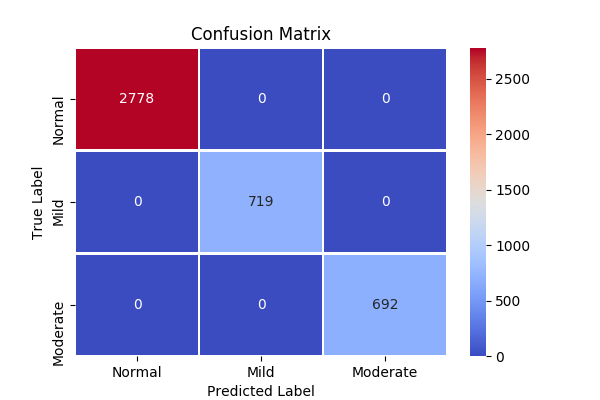
\includegraphics[height=8cm]{img/depression_class/conf_5760_60_50_32.png}
      \caption{50 epochs for 96 hour segments}
      \label{figure:depression_class_confusion_matrix_96h}
\end{figure}

\subsection{Training and finding the optimal segment length}

The next neural network we trained was for classifying how depressed the participants were. Depression classes are, as we said before, 
based on their MADRS score which is 0 for participants in the control group and differs between 11 and 28 in the condition group \ref{figure:demographics}. 
We labeled participants with MADRS score 0 as not depressed, between 11 and 19 as mildly depressed, and above 20 as moderately depressed. 

Using what we previously discovered from classifying control vs. condition groups, we knew how we wanted to achieve this goal. 
First, find the optimal segment length, then use the best segment length in cross-validation, and guarantee that the performance is consistent. 

In the previous experiment, there was a clear threshold after segment lengths of 24 hours where the performance didn't improve that much if increased more 
\ref{figure:control_condition_10e}. The results were just a little bit better for 48 than 24 hours and worse for longer segments. 
The question was whether the threshold existed for depression classes also, or if we could use longer segments to achieve better results.

We experimented the same way as before, except that we went straight for 50 epochs and skipped the shortest segments of 1, 2, 4 and 8 hours, 
as we were positive these segments would not be any good. We proceeded to train segment lengths of 16, 24, 48, 72 and 96 hours. 
Looking at the training and testing graphs \ref{figure:depression_class_50e}, we can see that the results for 96-hour segments were outstanding. 
We achieved an accuracy of 100\% on the testing set. The confusion matrix \ref{figure:depression_class_confusion_matrix_96h} shows not a single error in classification. 

\subsection{Cross-validation}

To make sure this wasn't just lucky, we needed to cross-validate here as well. We split the dataset into a training and testing set (80\%/20\%), 
then did three-fold cross-validation on the training set, just as before. If all three folds had similar accuracy and loss, and the mean values were good 
(close to 1.0 for accuracy and close to zero for loss), we had achieved a consistent model, and the model would be fit perfectly, 
at least for the 55 participants in the dataset. 

We trained the three models for 15 epochs each. We knew that wasn't enough to give us 100\% accuracy (need around 50 epochs for that), 
but we aimed for somewhere around 98-99\% for all folds. Looking at the cross-validation results \ref{figure:depression_class_cv}, we can see that the lowest 
accuracy was 98,5\% and the highest was 99,8\%. The mean accuracy for all three folds was 99\%, which is what we wanted to see. 

The model is indeed perfect for classifying depression classes, at least for all the participants in the dataset. We know that the model won't 
classify with 100\% accuracy on data outside the participants in the dataset since 55 persons can't possibly tell everything about human activity behavior, 
but you can read more on this later.

\begin{figure}
\begin{center}
      \begin{tabular}{|l|l|l|}
            \hline
            \bfseries Fold & \bfseries Loss & \bfseries Accuracy
            \csvreader[head to column names]{code/logs/depression_class/cv.csv}{}
            {\\\hline\fold & \loss & \accuracy}
            \\\hline
            \bfseries Mean & \bfseries 0.032561721418313254 & \bfseries 0.990689902124612
            \\\hline
      \end{tabular}
      \caption{3-Fold Cross validation}
      \label{figure:depression_class_cv}
\end{center}
\end{figure}

\section{1D CNN: MADRS Score Prediction}

\begin{figure}
      \begin{multicols}{2}
            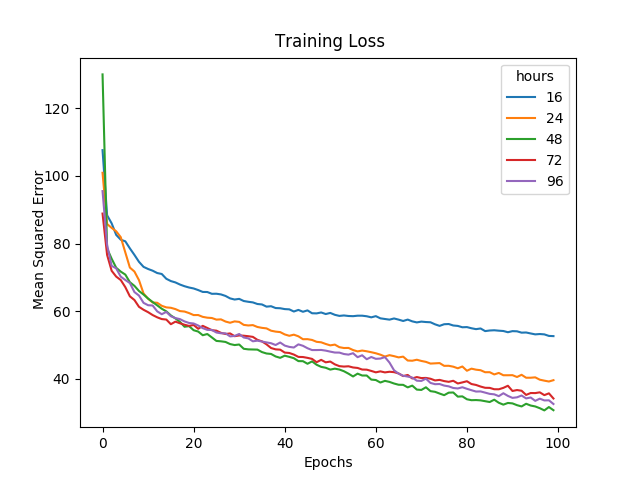
\includegraphics[height=5cm]{img/madrs_prediction/plot_loss_train.png}
            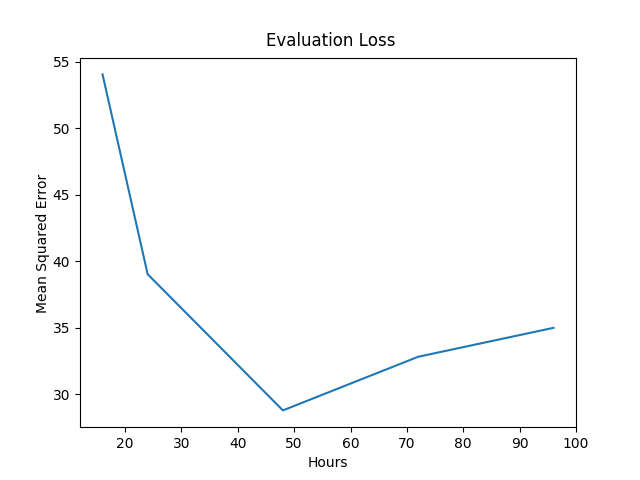
\includegraphics[height=5cm]{img/madrs_prediction/plot_loss_eval.png}
      \end{multicols}
      \caption{MADRS Prediction: Training (left) and testing (right) results (100 epochs)}
      \label{figure:madrs_prediction_50e}
\end{figure}

%\subsection{Performance metrics}
%\subsubsection{Accuracy}
%\subsubsection{Precision}
%\subsubsection{Recall}
%\subsubsection{Specificity}
%\subsubsection{F1 Score}
%\subsection{Cross validation}